
\documentclass{beamer}
\usetheme{ucl}

\usepackage[utf8]{inputenc}


%%% Increase the height of the banner: the argument is a scale factor >=1.0
%\setbeamertemplate{banner}[ucl][10.0]

%%% Change the colour of the main banner
%%% The background should be one of the UCL colours (except pink or white):
%%%   black,darkpurple,darkred,darkblue,darkgreen,darkbrown,richred,midred,
%%%   navyblue,midgreen,darkgrey,orange,brightblue,brightgreen,lightgrey,
%%%   lightpurple,yellow,lightblue,lightgreen,stone
\setbeamercolor{banner}{bg=darkpurple}
%\setbeamercolor{banner}{bg=yellow,fg=black}

%%% Add a stripe behind the banner
%\setbeamercolor{banner stripe}{bg=darkpurple,fg=black}

%%% The main structural elements
\setbeamercolor{structure}{fg=black}

%%% Author/Title/Date and slide number in the footline
\setbeamertemplate{footline}[author title date]

%%% Puts the section/subsection in the headline
% \setbeamertemplate{headline}[section]

%%% Puts a navigation bar on top of the banner
%%% For this to work correctly, the each \section command needs to be
%%% followed by a \subsection. Requires one extra compile.
% \setbeamertemplate{headline}[miniframes]
%%% Accepts an optional argument determining the width
% \setbeamertemplate{headline}[miniframes][0.3\paperwidth]


%%% Puts the frame title in the banner
%%% Won't work correctly with the above headline templates
%\useoutertheme{ucltitlebanner}
%%% Similar to above, but smaller (and puts subtitle on same line as title)
\useoutertheme[small]{ucltitlebanner}

%%% Gives block elements (theorems, examples) a border
% \useinnertheme{blockborder}
%%% Sets the body of block elements to be clear
% \setbeamercolor{block body}{bg=white,fg=black}

%%% Include CSML logo on title slide
%\titlegraphic{\includegraphics[width=0.16\paperwidth]{csml_logo}}

%%% Include CSML logo in bottom right corner of all slides
%\logo{\includegraphics[width=0.12\paperwidth]{csml_logo}}

%%% Set a background colour
% \setbeamercolor{background canvas}{bg=lightgrey}

%%% Set a background image
%%% Some sample images are available from the UCL image store:
%%%   https://www.imagestore.ucl.ac.uk/home/start
% \setbeamertemplate{background canvas}{%
%   \includegraphics[width=\paperwidth]{imagename}}



%%%%%% Some other settings that can make things look nicer
%%% Set a smaller indent for description environment
\setbeamersize{description width=2em}
%%% Remove nav symbols (and shift any logo down to corner)
\setbeamertemplate{navigation symbols}{\vspace{-2ex}}








\DeclareMathOperator{\Cov}{Cov}
\DeclareMathOperator{\Var}{Var}
\DeclareMathOperator{\E}{\mathbb{E}}
\DeclareMathOperator{\Proba}{\mathbb{P}}

\newcommand{\Covb}[2]{\ensuremath{\Cov\!\left[#1,#2\right]}}
\newcommand{\Eb}[1]{\ensuremath{\E\!\left[#1\right]}}
\newcommand{\Pb}[1]{\ensuremath{\Proba\!\left[#1\right]}}
\newcommand{\Varb}[1]{\ensuremath{\Var\!\left[#1\right]}}

% norm
\newcommand{\norm}[1]{\| #1 \|}

\newcommand{\indep}{\rotatebox[origin=c]{90}{$\models$}}





\usepackage{mathptmx,amsmath,amssymb,graphicx,bibentry,bbm,ragged2e}
\usepackage[english]{babel}

\makeatletter

\newcommand{\noun}[1]{\textsc{#1}}
\newcommand{\jitem}[1]{\item \begin{justify} #1 \end{justify} \vfill{}}
\newcommand{\sframe}[2]{\frame{\frametitle{#1} #2}}

\newenvironment{centercolumns}{\begin{columns}[c]}{\end{columns}}
%\newenvironment{jitem}{\begin{justify}\begin{itemize}}{\end{itemize}\end{justify}}



%\usetheme{Warsaw}
%\setbeamertemplate{footline}[text line]{}
%\setbeamertemplate{headline}{}
%\setbeamercolor{structure}{fg=purple!50!blue, bg=purple!50!blue}

%\setbeamersize{text margin left=15pt,text margin right=15pt}

%\setbeamercovered{transparent}


\@ifundefined{showcaptionsetup}{}{%
 \PassOptionsToPackage{caption=false}{subfig}}
\usepackage{subfig}

\usepackage[utf8]{inputenc}
\usepackage[T1]{fontenc}

\usepackage{multirow}


\makeatother

\def \draft {1}

\usepackage{xparse}
\usepackage{ifthen}
\DeclareDocumentCommand{\comment}{m o o o o}
{\ifthenelse{\draft=1}{
    \textcolor{red}{\textbf{C : }#1}
    \IfValueT{#2}{\textcolor{blue}{\textbf{A1 : }#2}}
    \IfValueT{#3}{\textcolor{ForestGreen}{\textbf{A2 : }#3}}
    \IfValueT{#4}{\textcolor{red!50!blue}{\textbf{A3 : }#4}}
    \IfValueT{#5}{\textcolor{Aquamarine}{\textbf{A4 : }#5}}
 }{}
}
\newcommand{\todo}[1]{
\ifthenelse{\draft=1}{\textcolor{red!50!blue}{\textbf{TODO : \textit{#1}}}}{}
}




\begin{document}


\title[Integrating urban models]{Integrating and validating urban simulation models}

\author[J.~Raimbault]{J.~Raimbault$^{1,2,3\ast}$\\
\texttt{j.raimbault@ucl.ac.uk}
}


\institute[UCL]{$^{1}$CASA, UCL\\
$^{2}$UPS CNRS 3611 Complex Systems Institute Paris\\
$^{3}$UMR CNRS 8504 G{\'e}ographie-cit{\'e}s
}


\date[28/05/2021]{French Regional Conference on Complex Systems\\
May 28th 2021\\\smallskip

\includegraphics[width=0.1\textwidth]{figures/logoFRCCS}
}

\frame{\maketitle}


% Juste Raimbault holds a PhD from University Paris 7 in Quantitative Geography, on modeling the co-evolution of transportation networks and territories. With an interdisciplinary background in Complex Systems, his work is situated at the interface of Geography and Computer Science. He is currently a Research Fellow at the Center for Advanced Spatial Analysis, University College London, where he studies the coupling of microsimulation models with land-use transport interaction models. He is also an associate researcher at Institut des Systèmes Complexes Paris Ile-de-France, where he develops model exploration and validation methods and contributes to the development of the OpenMOLE platform.




\sframe{Modeling urban complexity}{


\textit{Large scale urban models are intrinsically flawed and do not reach their goals of long-term application to planning}: \textbf{Requiem for large scale models in 1973} \cite{lee1973requiem}

\bigskip


\textit{Urban analytics and Smart Cities approaches may follow the same path if they ignore the past and the complexity of cities} \cite{batty2014can}


\bigskip


To foster relevance of large urban models:

\begin{itemize}
	\item Transparency on data and implementation, reproducibility
	\item Validation of models and sub-models: from small simple models well validated to larger integrated models
\end{itemize}

\medskip

$\rightarrow$ Open, reproducible urban models can be shared, coupled into modular integrated models, tested and validated \cite{banos2013pour}

}

\sframe{Towards integrated urban models}{

\justify

\textbf{Research project}

\smallskip

\textit{Constructing urban models integrating disciplines and scales following the complex systems roadmap \cite{bourgine2009french}, towards an application to sustainable multi-scale policies}

\bigskip

$\rightarrow$ Horizontal integration (model coupling and interdisciplinarity)

\medskip

$\rightarrow$ Vertical integration (multi-scale models)

\medskip

$\rightarrow$ Model exploration and validation methods


}




\sframe{Interactions between networks and territories}{

\justify

\begin{center}
\includegraphics[width=0.45\linewidth]{figures/accessp_withbridge_prd_EN.png}
\hspace{0.1cm}
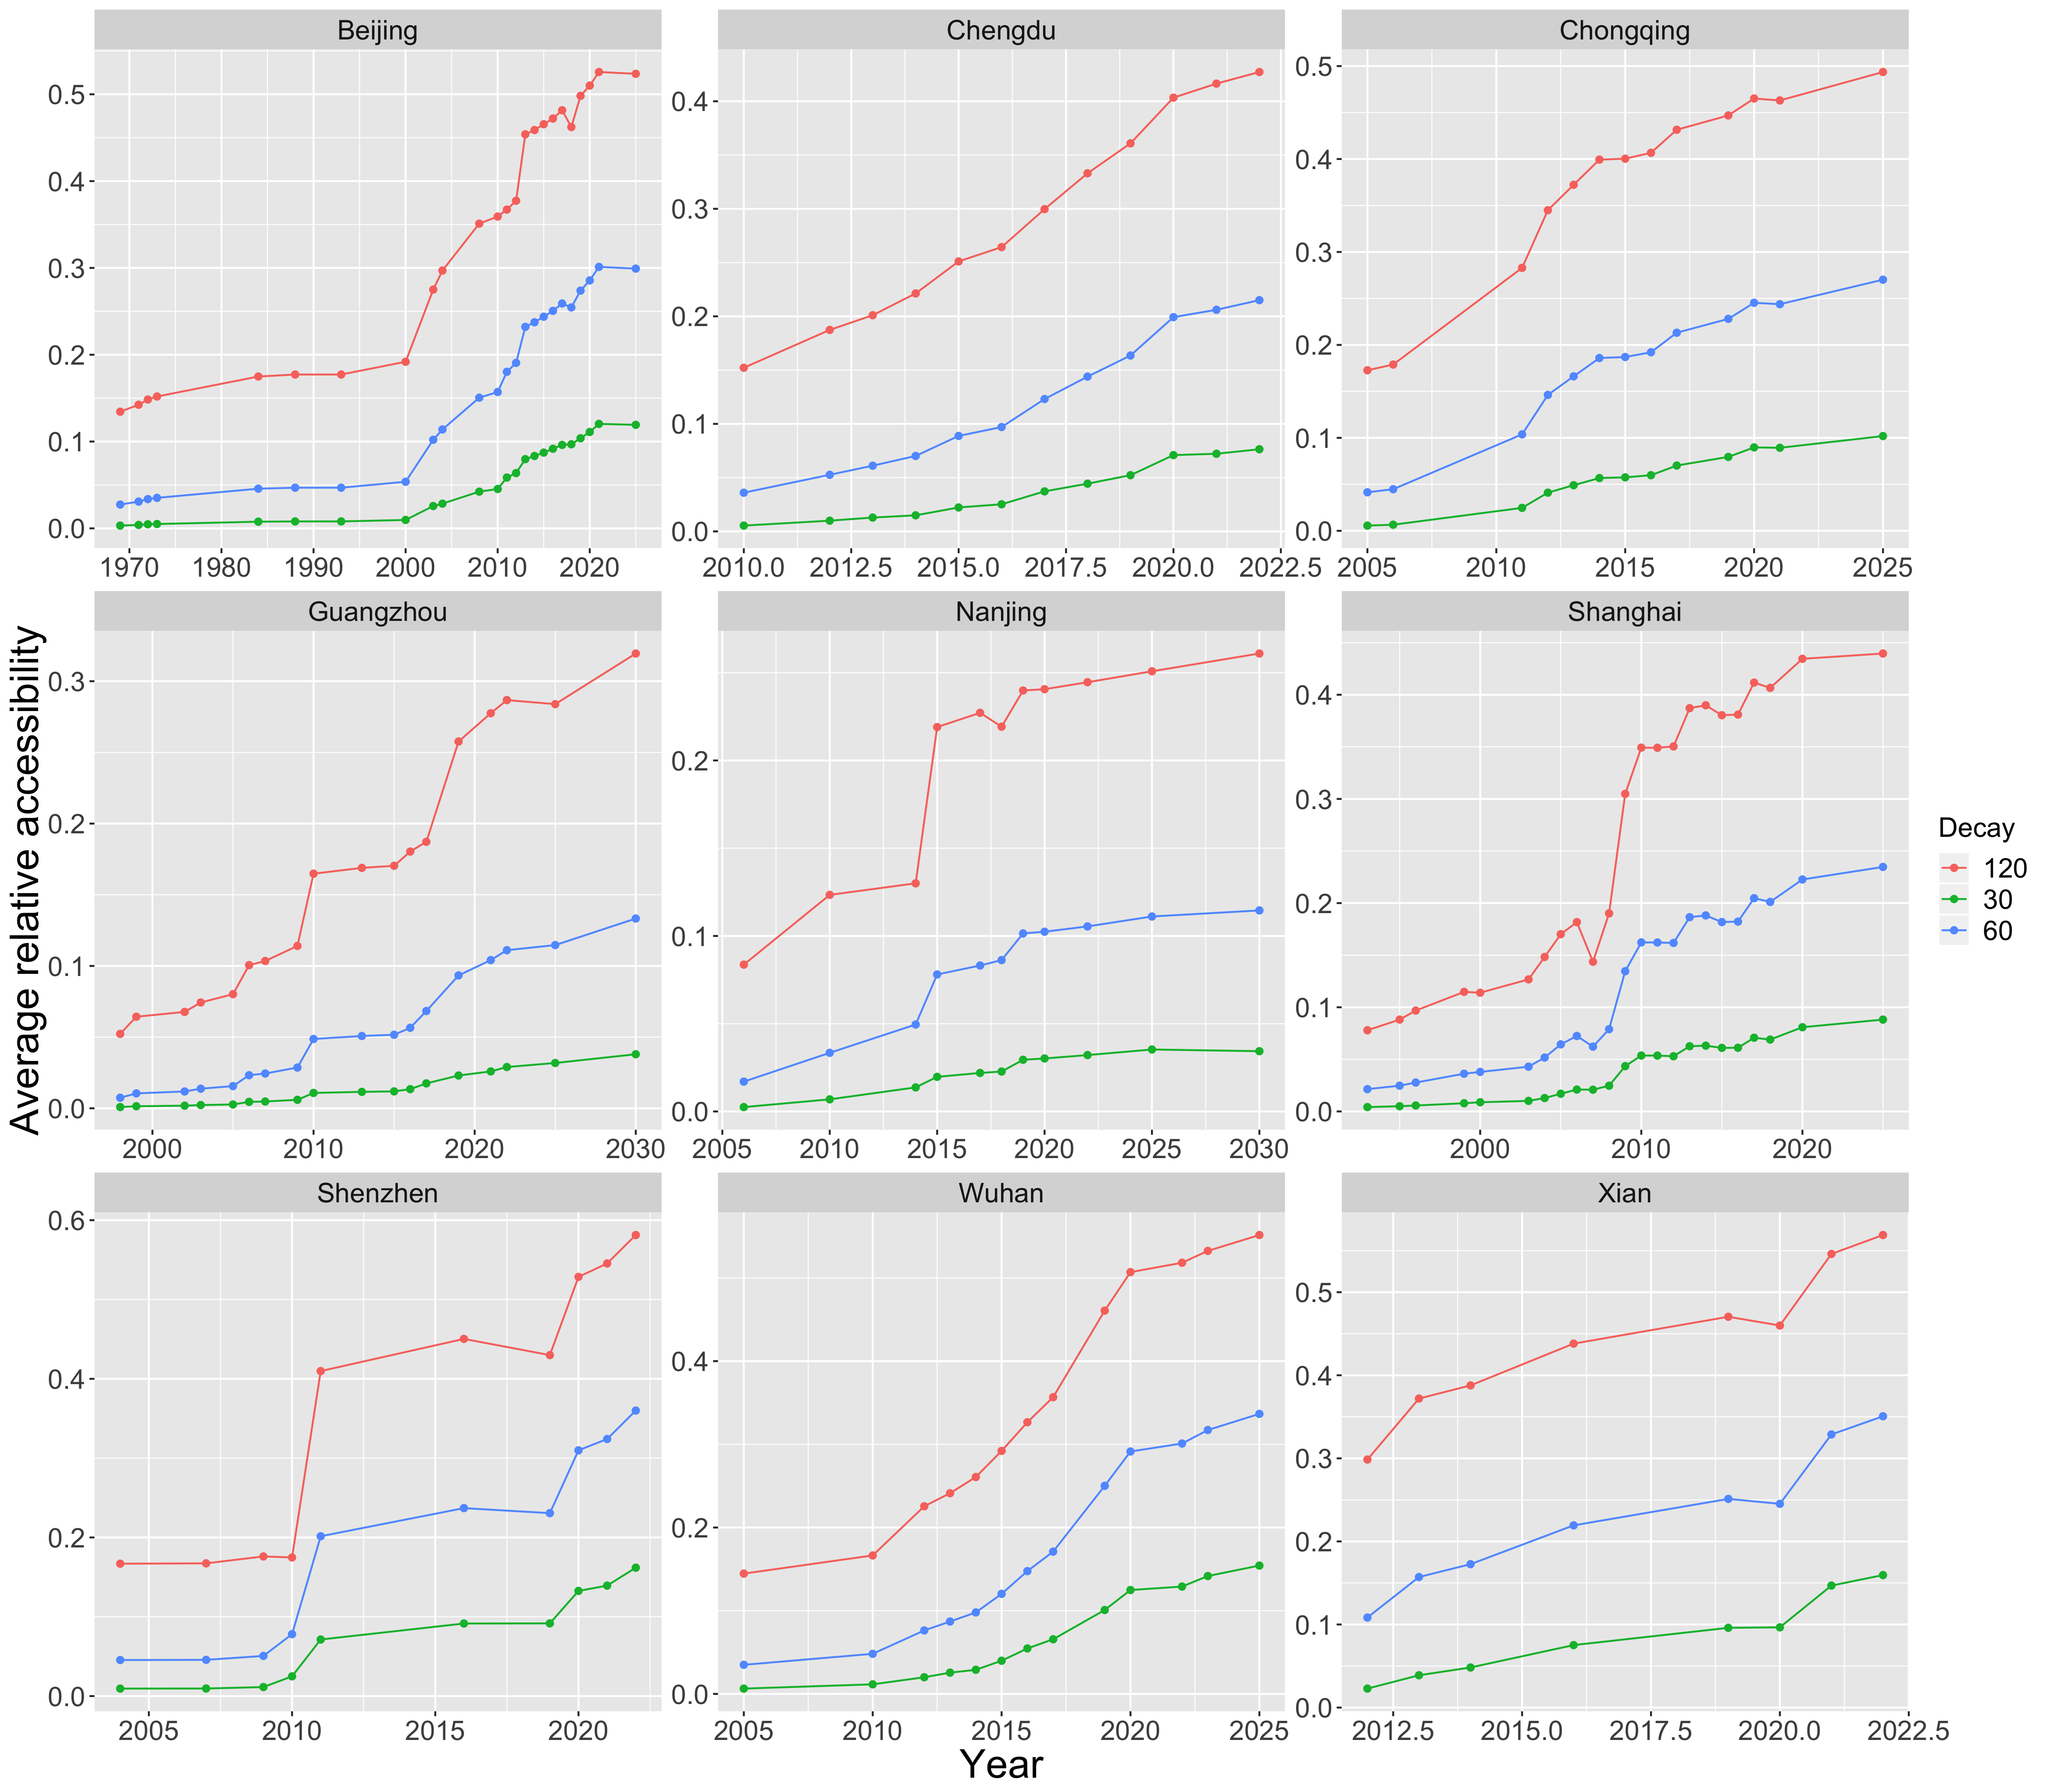
\includegraphics[width=0.52\linewidth]{figures/avgaccess_facet.png}

\end{center}

\medskip

%\vspace{-0.5cm}

%\begin{justify}
\textit{Accessibility as part of complex processes of co-evolution between transportation networks and territories.}

%\end{justify}

\nocite{raimbault2018evolving}

\medskip

\tiny

Raimbault, J. (2019). Evolving accessibility landscapes: mutations of transportation networks in China. In Aveline-Dubach, N., ed. \textit{Pathways of sustainable urban development across China - the cases of Hangzhou, Datong and Zhuhai}, pp 89-108. Imago. ISBN:978-88-94384-71-0

}



\sframe{Mesoscopic models: morphogenesis}{



\footnotesize

\justify
\textit{A morphogenesis model with reaction-diffusion and multi-modeling of network growth: complementarity of heuristics, calibration for Europe on forms and their correlations}

\smallskip

\begin{center}
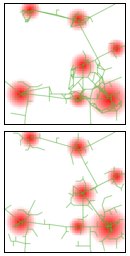
\includegraphics[width=0.25\linewidth,height=0.6\textheight]{figures/meso-nwgrowth.png}
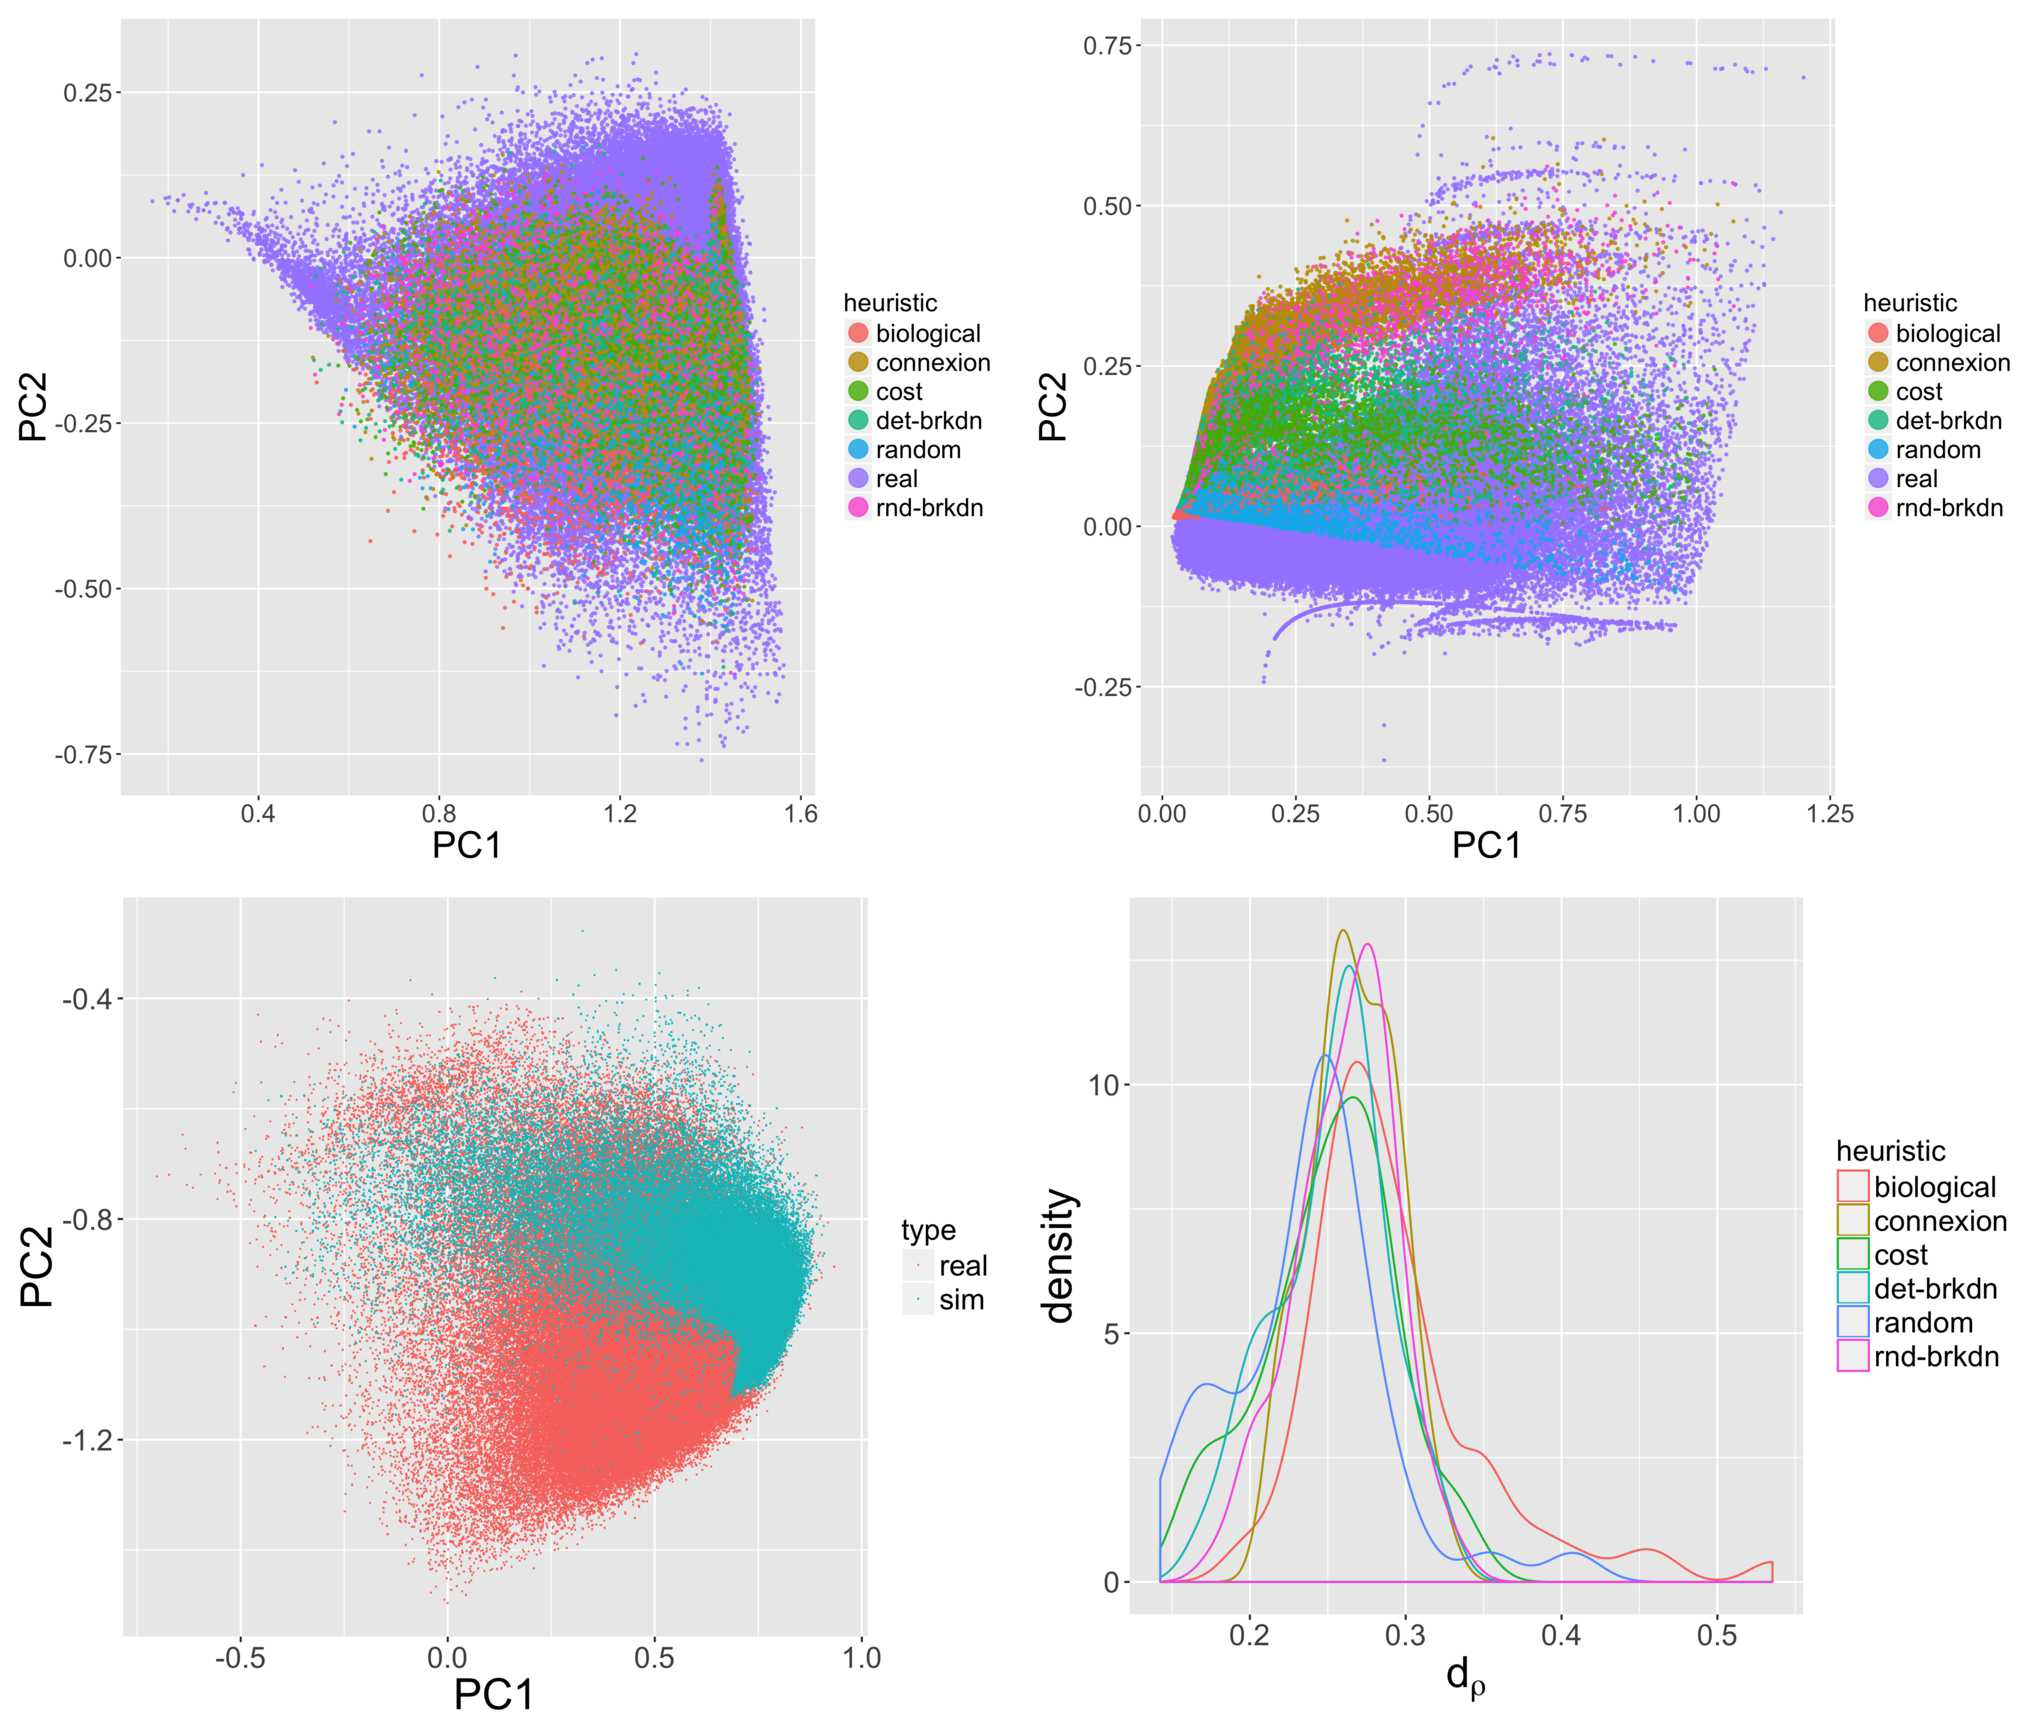
\includegraphics[width=0.6\linewidth,height=0.6\textheight]{figures/meso-calib.jpg}
\end{center}


\smallskip

\tiny

Raimbault, J. (2018). Calibration of a density-based model of urban morphogenesis. PloS one, 13(9), e0203516.

\nocite{raimbault2018calibration}

\smallskip

Raimbault, J. (2019). An urban morphogenesis model capturing interactions between networks and territories. In The Mathematics of Urban Morphology (pp. 383-409). Birkhäuser, Cham.

\nocite{raimbault2019urban}

}







\sframe{Macroscopic interaction model}{

\textit{System of cities interaction model including network evolution; production of multiple co-evolution regimes and calibration for France.}

\medskip

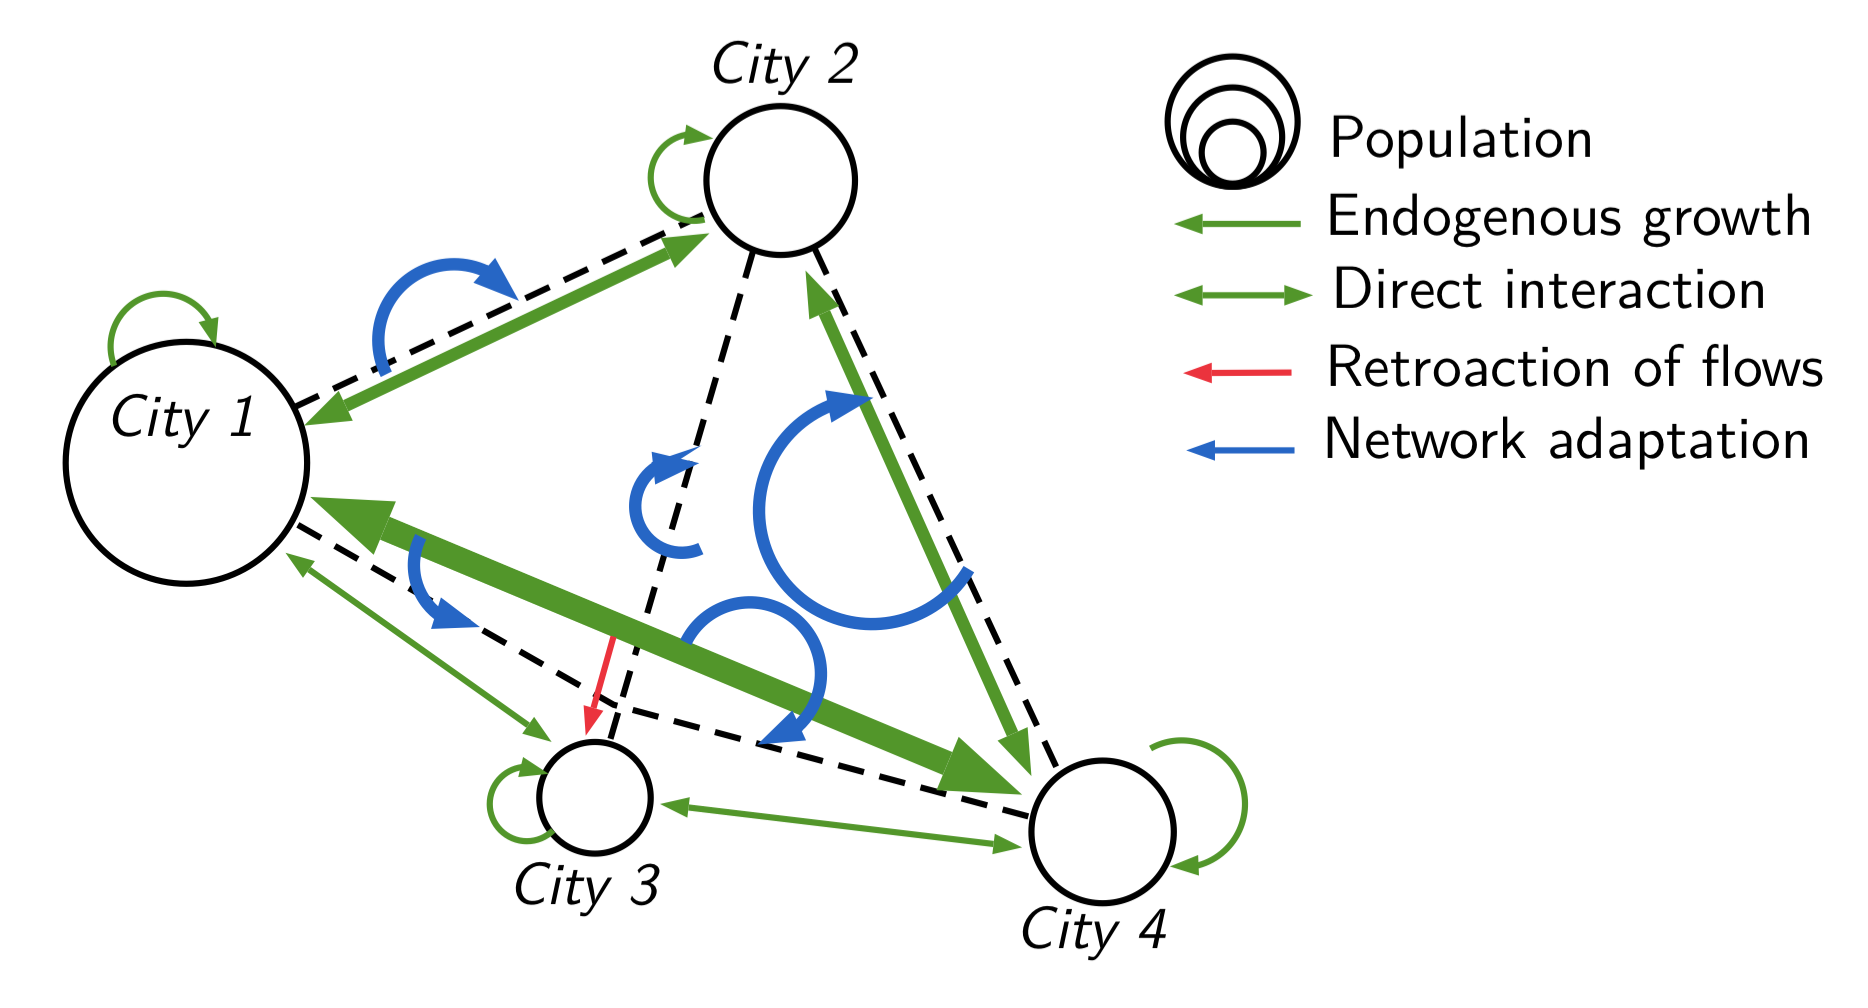
\includegraphics[width=0.6\textwidth]{figures/macrocoevol_en.png}
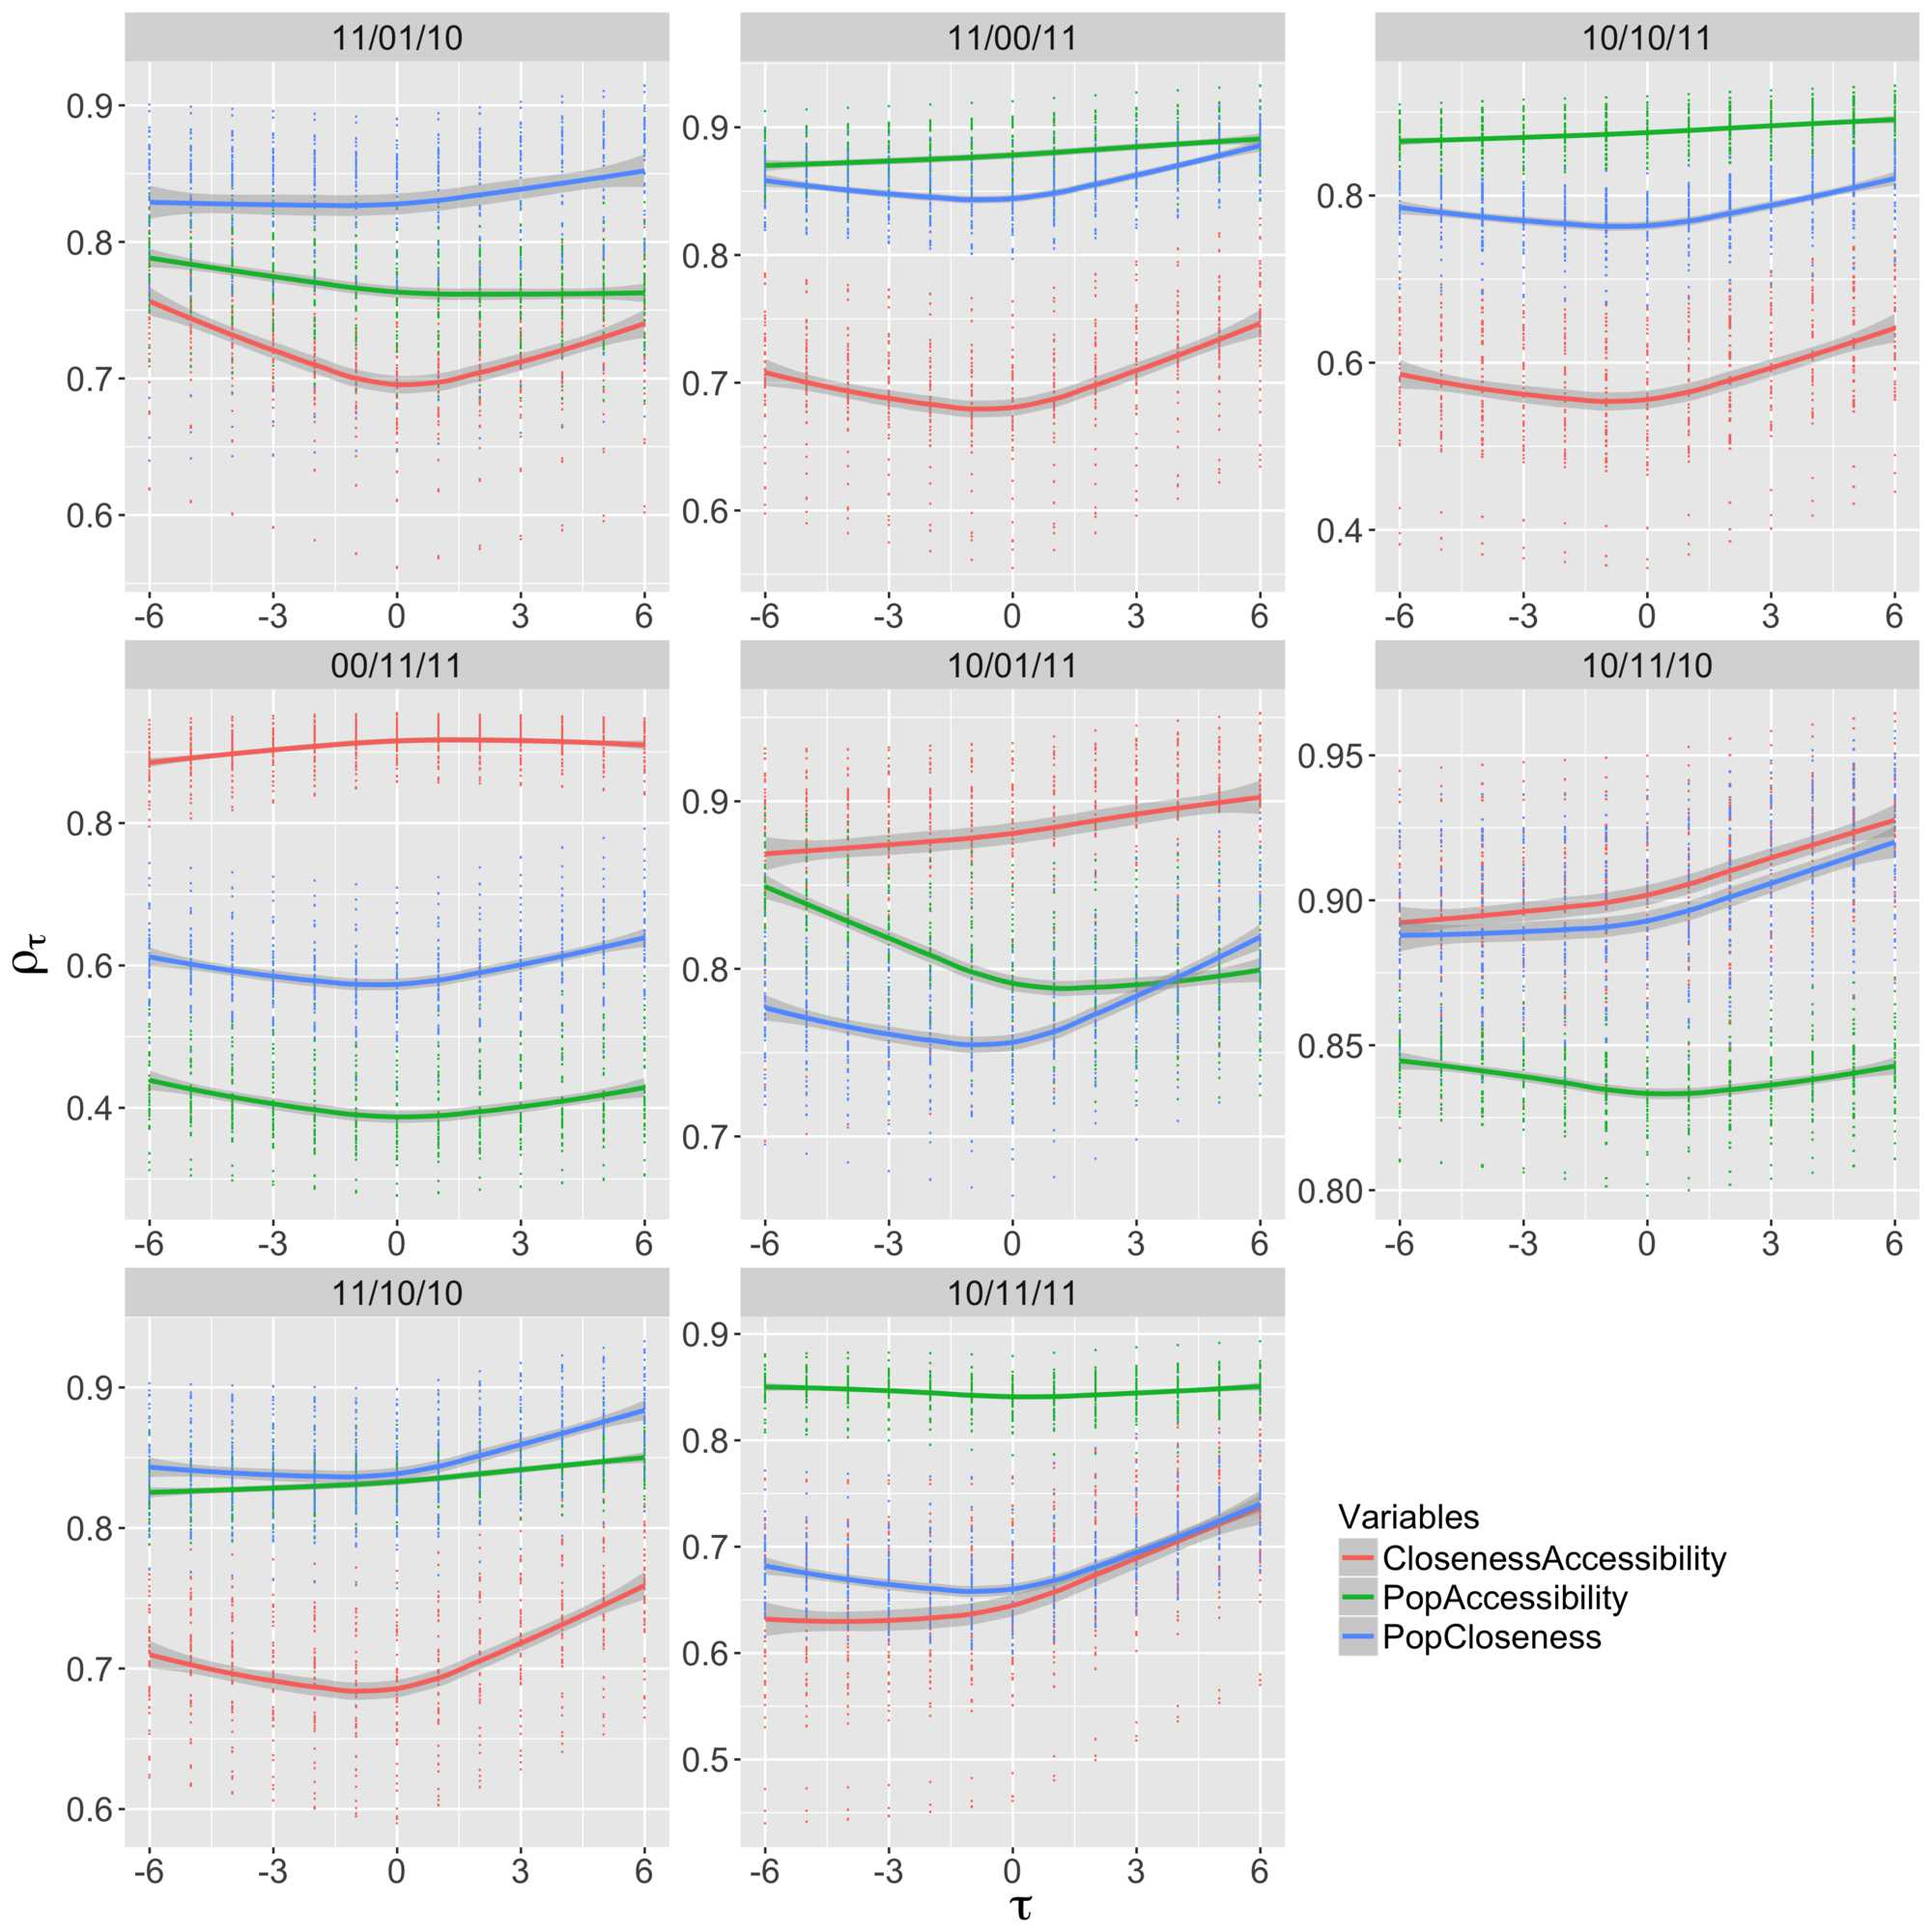
\includegraphics[width=0.39\linewidth]{figures/6-2-2-fig-macrocoevol-correlations.jpg}


\nocite{raimbault2020indirect}
\nocite{raimbault2021modeling}


\bigskip

\tiny

Raimbault, J. (2020). Indirect evidence of network effects in a system of cities. Environment and Planning B: Urban Analytics and City Science, 47(1), 138-155.

\smallskip

Raimbault, J. (2021). Modeling the co-evolution of cities and networks. In Niel, Z., Rozenblat, C., eds. \textit{Handbook of Cities and Networks}, Edwar Elgar Publishing, \textit{in press}.


}




\sframe{Horizontal integration: interdisciplinarity}{

\textit{Literature mapping and systematic review tools to enhance integration}

\medskip

\begin{center}
	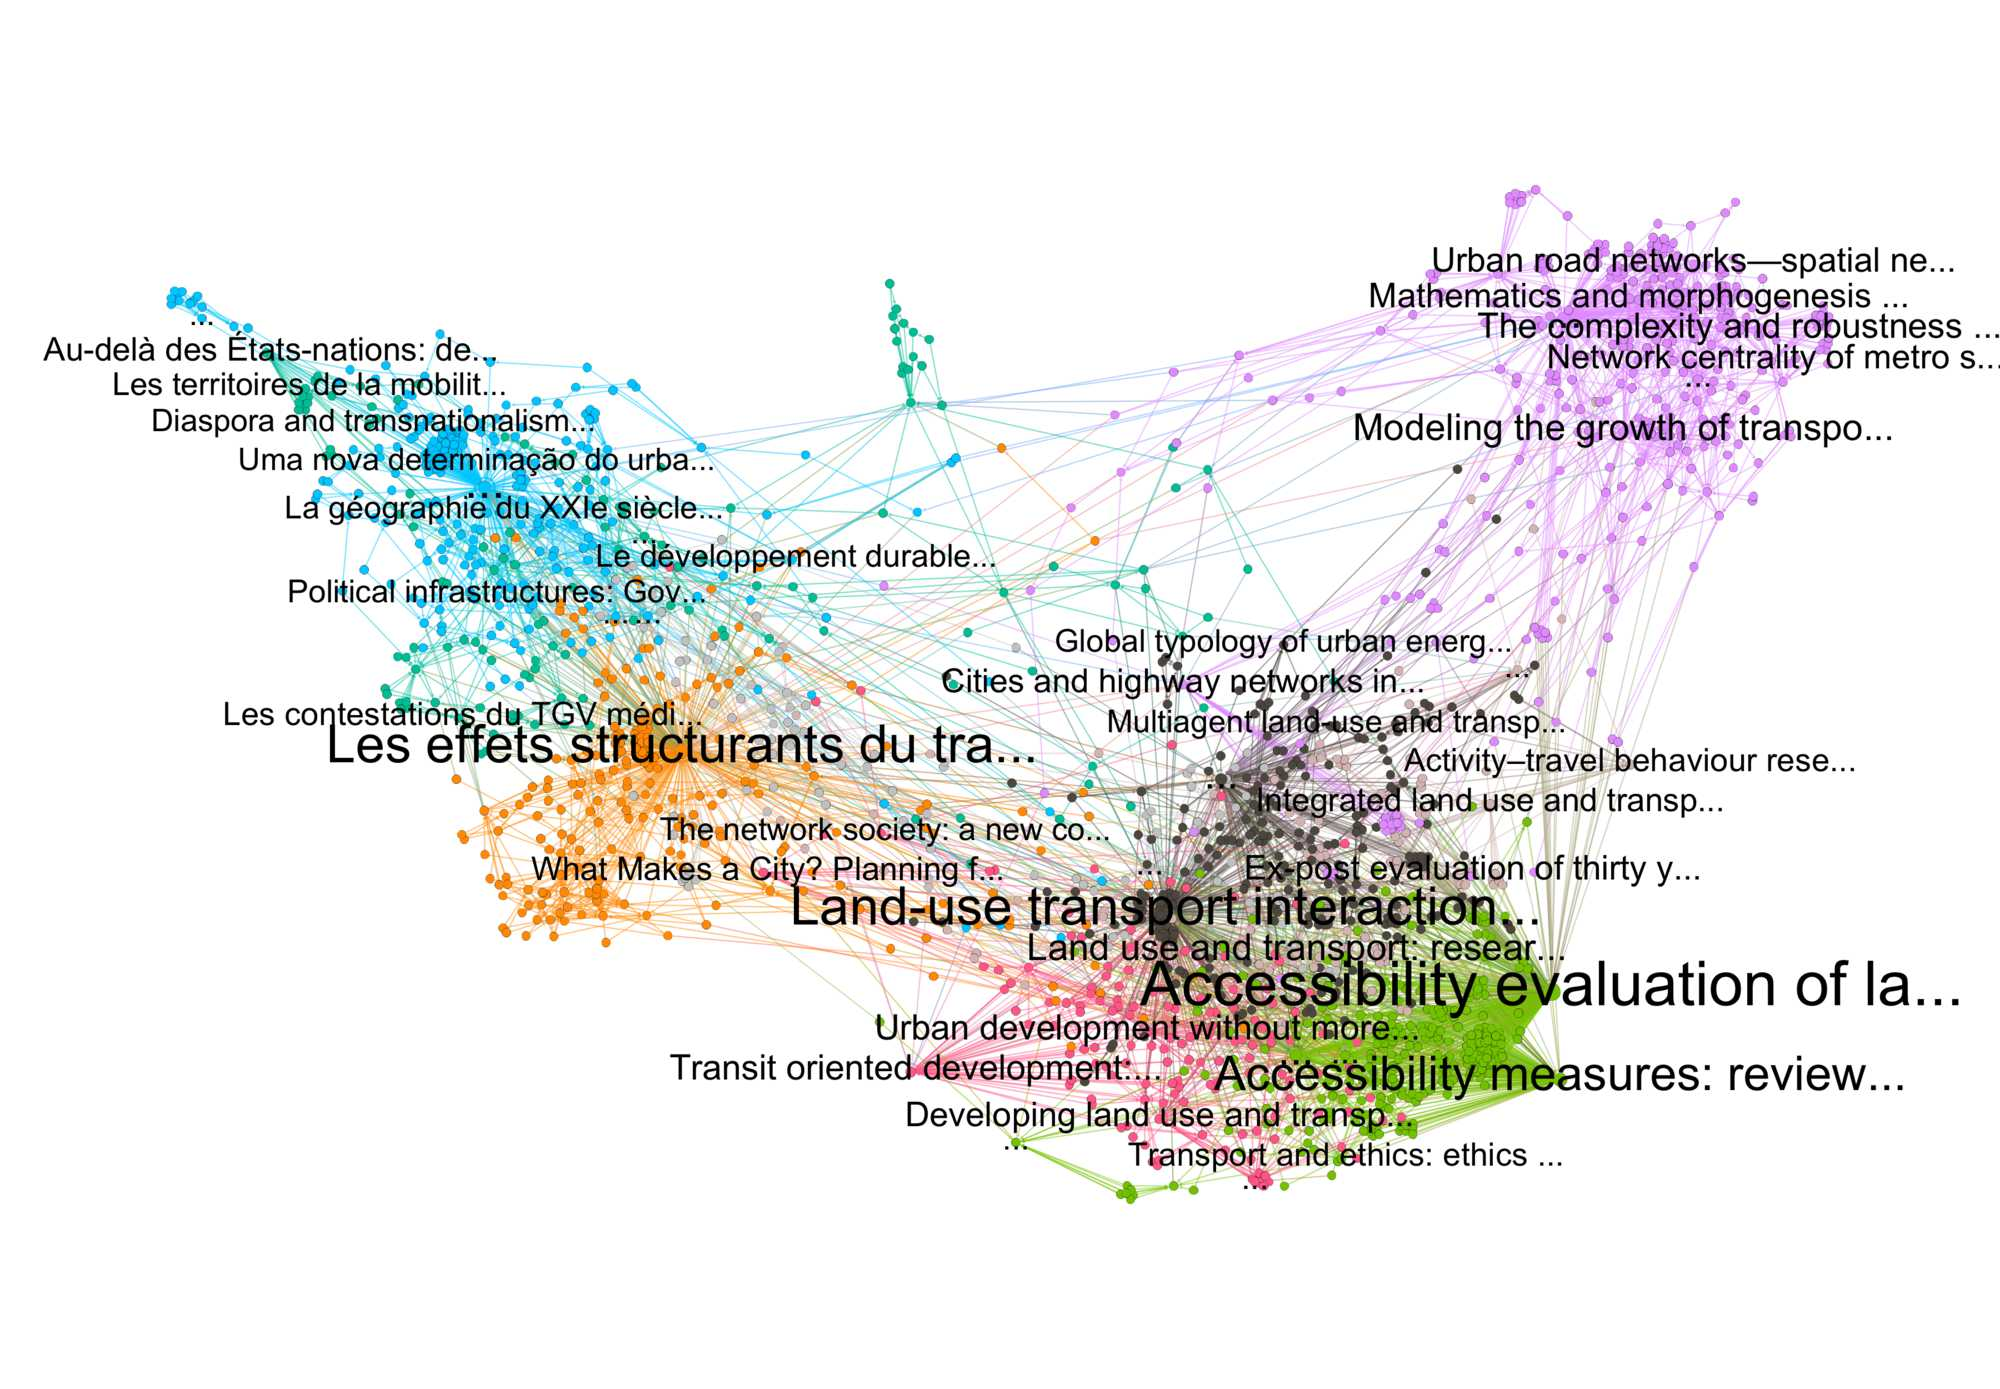
\includegraphics[width=0.9\textwidth,trim={0 2cm 0 2cm},clip]{figures/2-2-2-fig-quantepistemo-citnw.jpg}	
\end{center}

\medskip

\tiny

\vspace{-1cm}

Raimbault, J. (2019). Exploration of an interdisciplinary scientific landscape. Scientometrics, 119(2), 617-641.

\nocite{raimbault2019exploration}

}


\sframe{Building modular open transport models}{


\textbf{Case study:} \textit{Construct a modular four-step multimodal transportation model using open source projects and data}

\bigskip

\textbf{Integrated models:}

\begin{itemize}
	\item MATSim model (MATSim Community) for the transportation system \url{https://www.matsim.org/} \cite{horni2016multi}
	\item SPENSER model (University of Leeds) for the synthetic population \url{https://github.com/nismod/microsimulation}
	\item QUANT model (CASA, University College London) for spatial interactions to generate home-work plans \url{http://quant.casa.ucl.ac.uk/} \cite{milton2019accelerating}
	\item spatialdata library (OpenMOLE community) for data processing \url{https://github.com/openmole/spatialdata} \cite{raimbault2020scala}
\end{itemize}



}


\sframe{Issues when coupling models}{

\begin{table}
\vspace{-0.7cm}
	\centering
	\begin{tabular}{|p{3.8cm}|p{3.5cm}|p{3.5cm}|}
	\hline
	\footnotesize
	& QUANT & SPENSER \\
	\hline
Time scale & 10 years & 40 years \\
Spatial scale & UK & UK \\
Spatial resolution & MSOA & MSOA \\
Agent granularity & Aggregated counts & individual level \\
Static/Dynamic & Equilibrium (static) & Dynamic \\
Randomness & Deterministic & Monte-Carlo \\\hline
Transportation & 3 modes & NA \\
Economics & Accessibility-based relocations & NA \\
Demographics & NA & Data-driven \\
Migration flows & Accessibility-based relocations & Data-driven \\
\hline
	\end{tabular}
\end{table}

\smallskip

\footnotesize

\begin{itemize}
	\item Weak coupling Luti $\rightarrow$ microsimulation
	\item Weak coupling Microsimulation $\rightarrow$ Luti
	\item Strong coupling: as much choices as potential ``coupling processes''
\end{itemize}

}



\sframe{Vertical integration: multi-scale models}{


\textit{Processes specific to scales, coupling requires dedicated ontologies} 


\bigskip

\begin{center}
	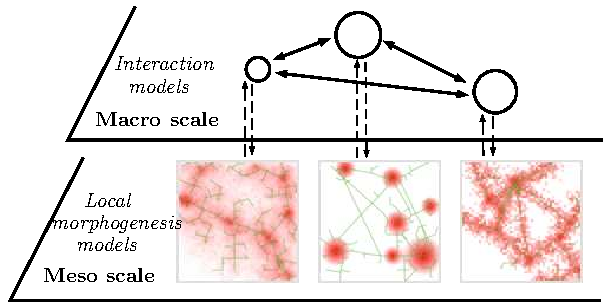
\includegraphics[width=0.9\textwidth]{figures/multiscale_morph.pdf}
\end{center}

\nocite{raimbault2021strong}

\tiny

Raimbault, J. (2021). Strong coupling between scales in a multi-scalar model of urban dynamics. arXiv preprint arXiv:2101.12725.

}





\sframe{Model exploration methods to foster knowledge integration}{
	
	OpenMOLE software \cite{reuillon2013openmole}: \textit{(i) Innovative exploration methods; (ii) Scaling of methods on high performance computing environments; (iii) Scripts to embed and couple models.}
	
	\smallskip
	
	\centering
	
	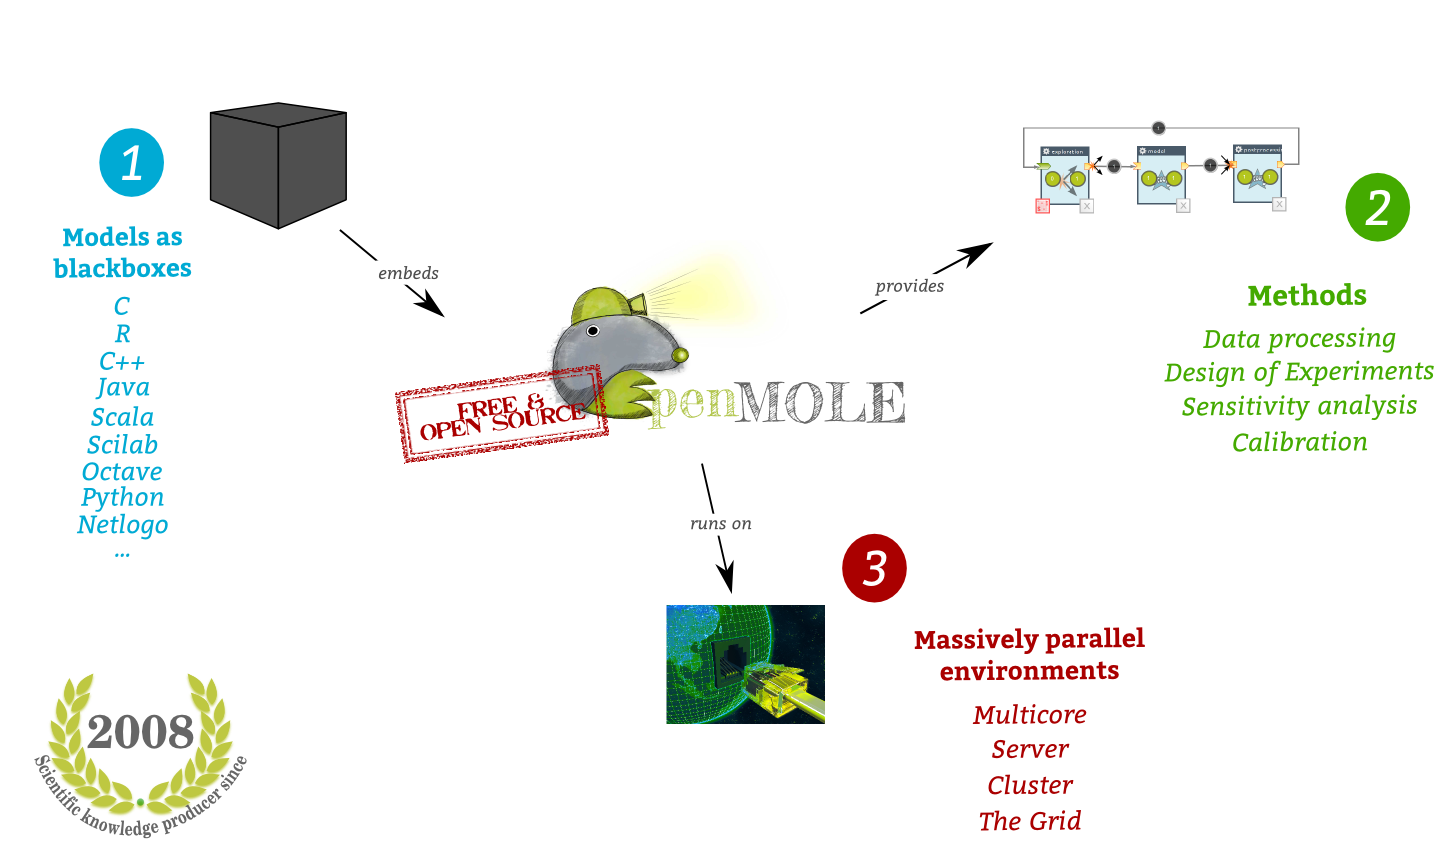
\includegraphics[width=0.8\textwidth]{figures/openmoleGal.png}
	
}




\sframe{Validation: towards spatial sensitivity analysis}{



\centering

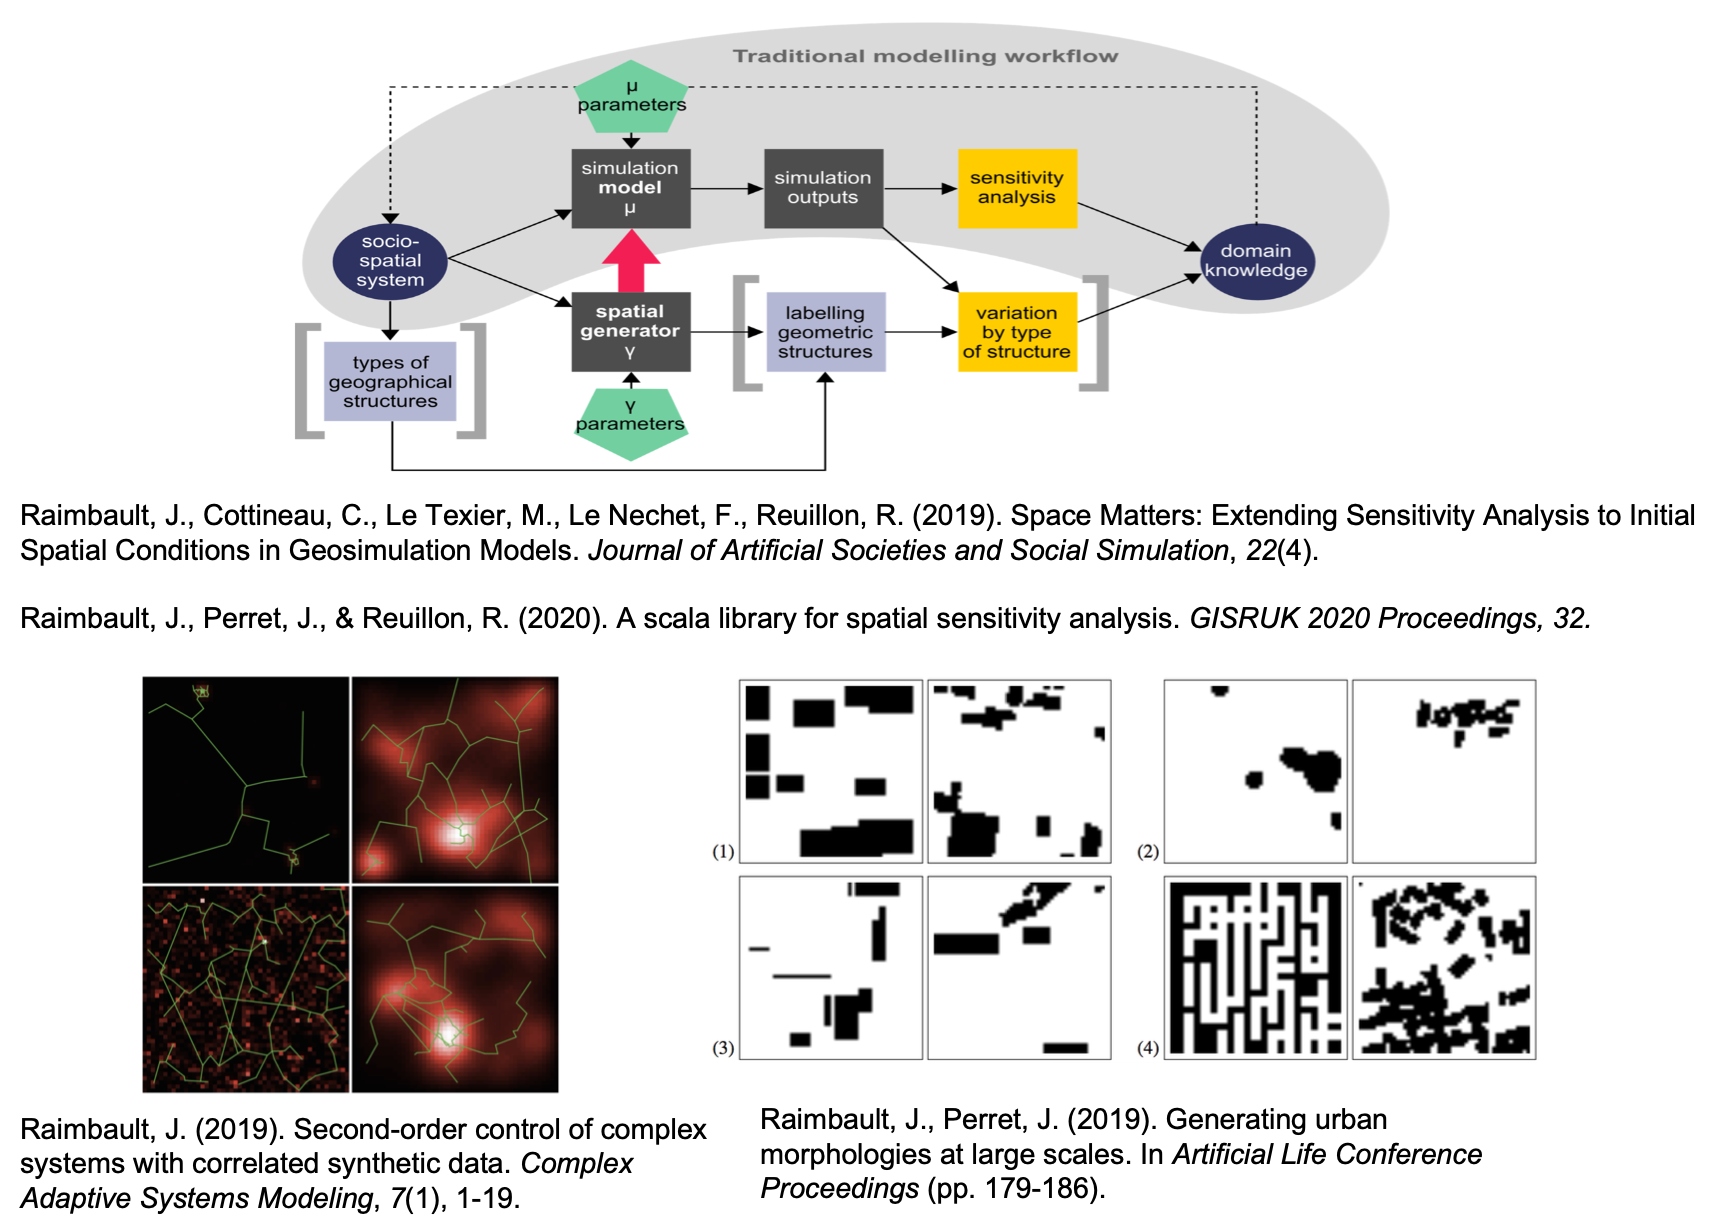
\includegraphics[width=0.95\linewidth]{figures/spatial_sa.png}

\nocite{raimbault2019second}
\nocite{raimbault2019generating}
\nocite{raimbault2019space}

}





\sframe{Towards models for sustainable policies}{


\textit{Benchmark of growth models for systems of cities} 

\begin{center}
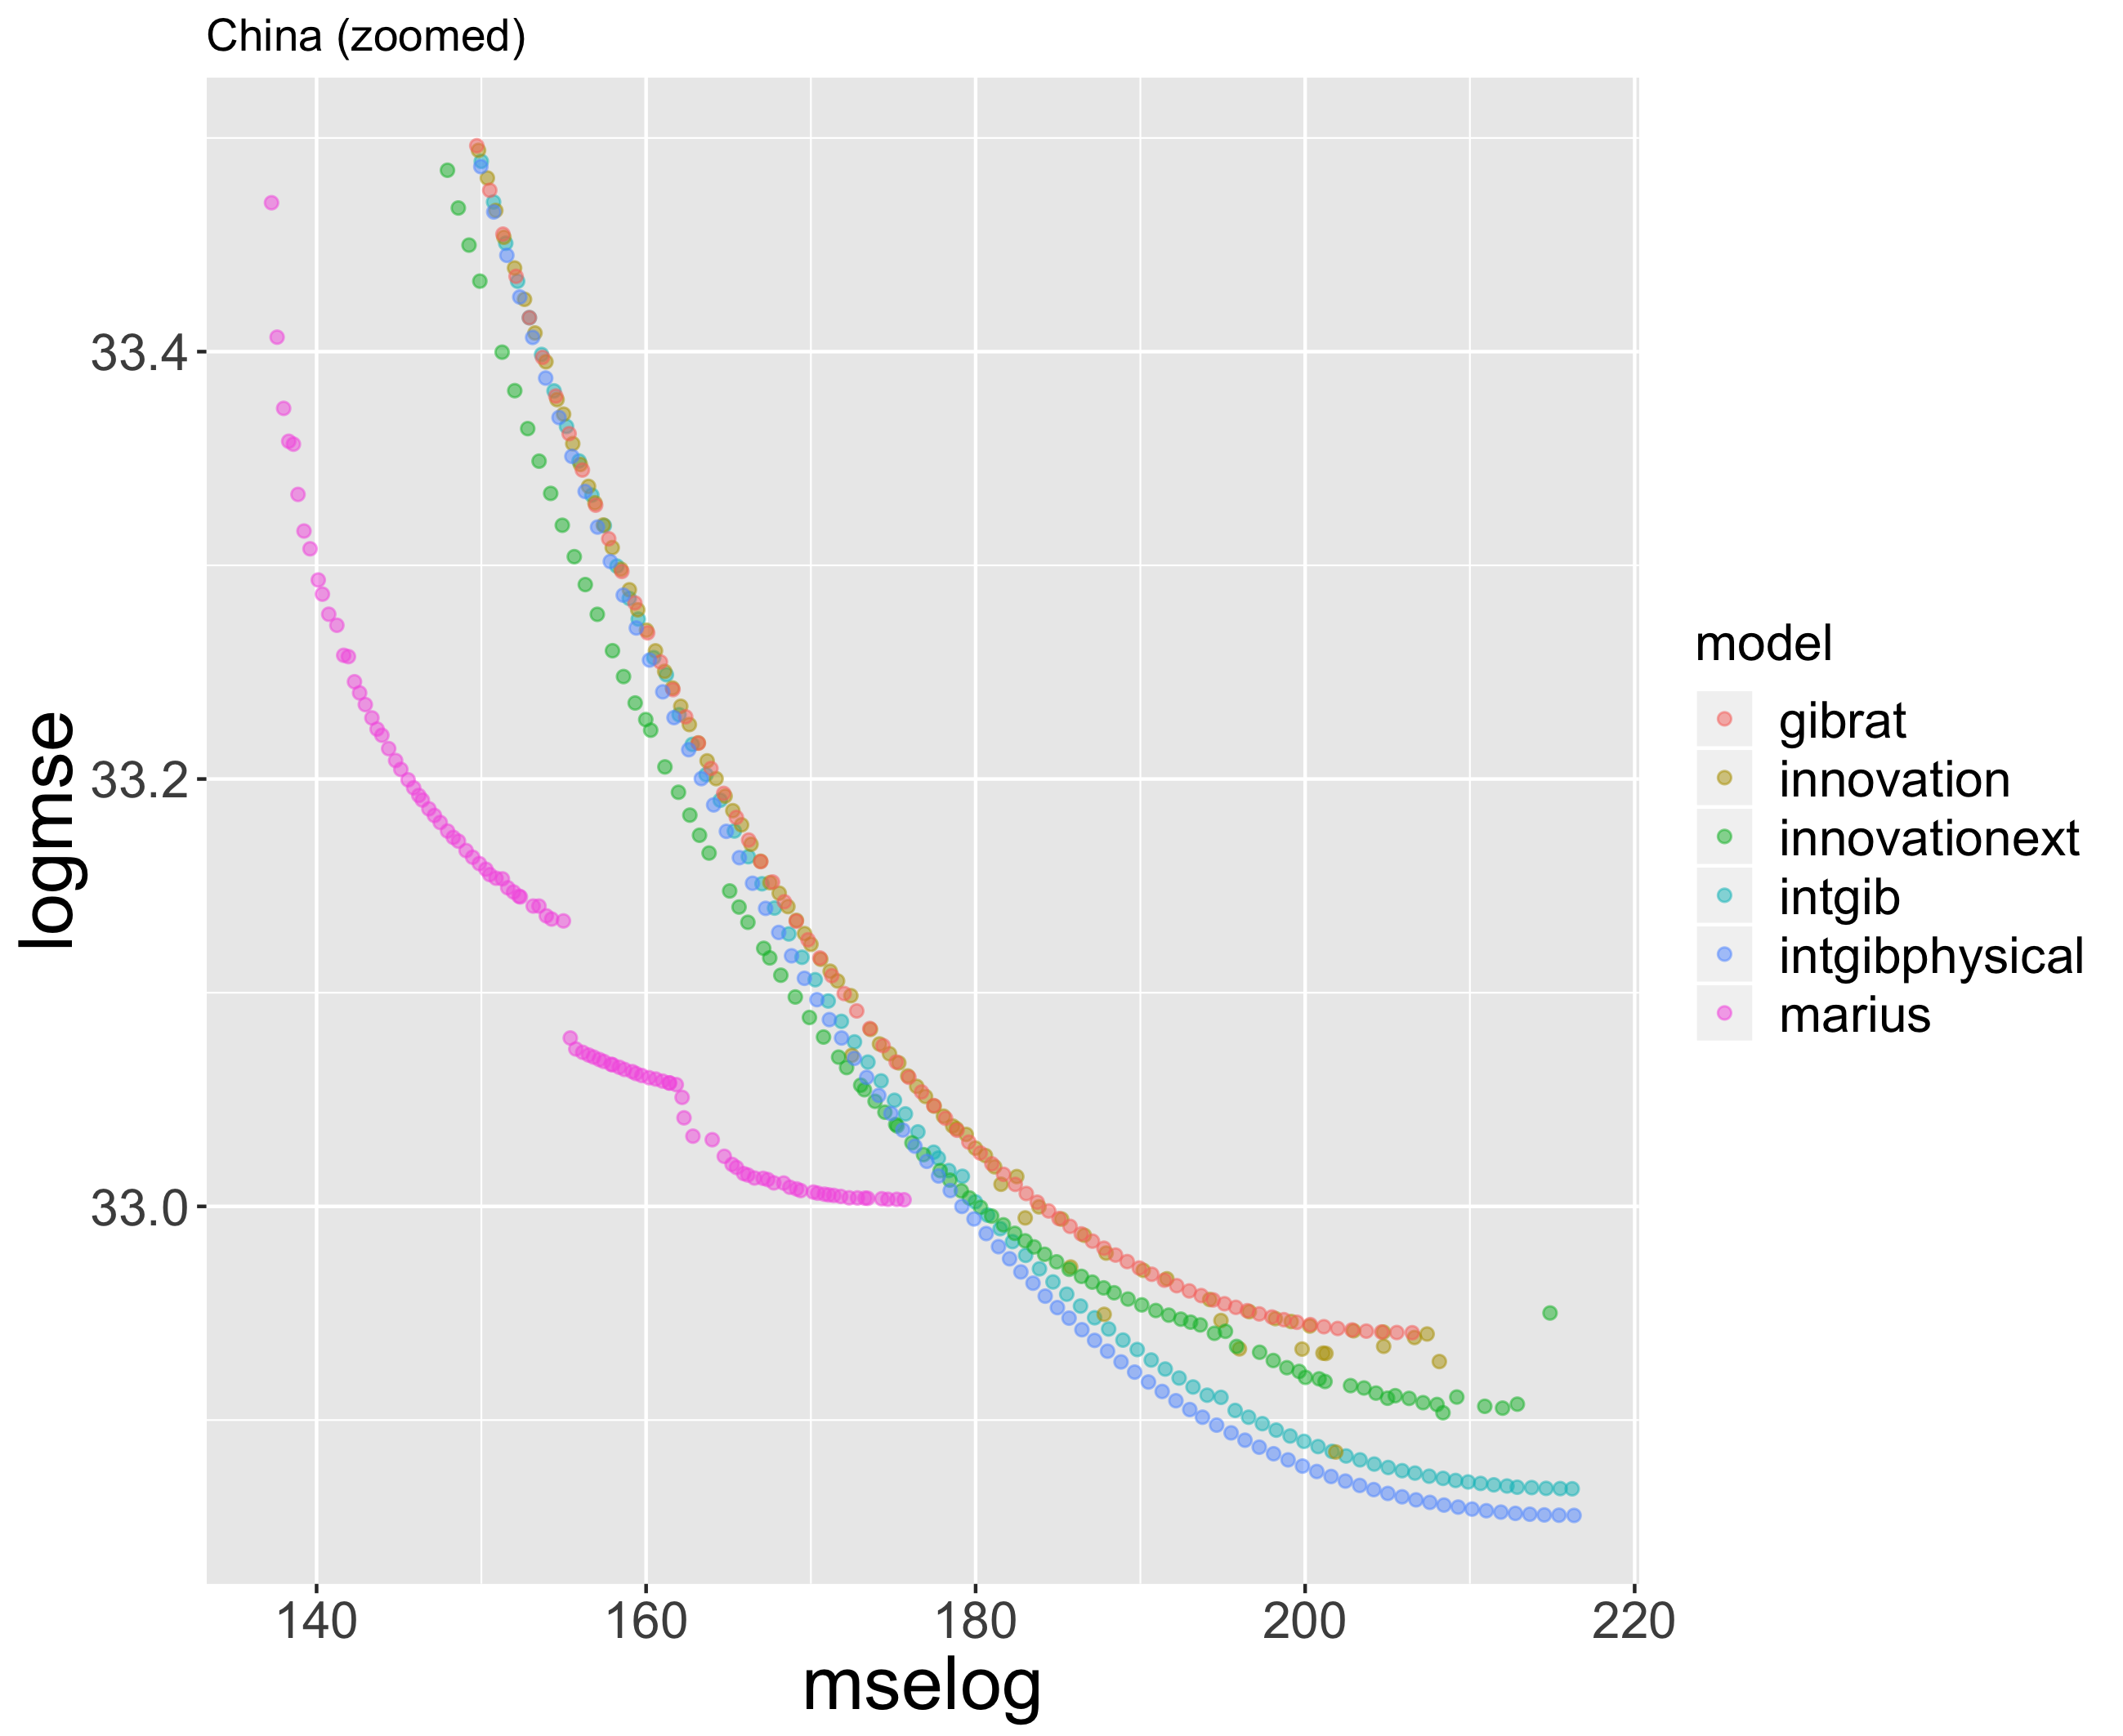
\includegraphics[width=0.65\textwidth]{figures/CN_zoomed.png}
\end{center}

\tiny

Raimbault, J., Denis, E., \& Pumain, D. (2020). Empowering Urban Governance through Urban Science: Multi-Scale Dynamics of Urban Systems Worldwide. Sustainability, 12(15), 5954.

\nocite{raimbault2020empowering}

}


\sframe{Towards models for sustainable policies}{

\textit{Identifying endogenous sustainable mega-city regions in Europe}

\medskip

% Marami
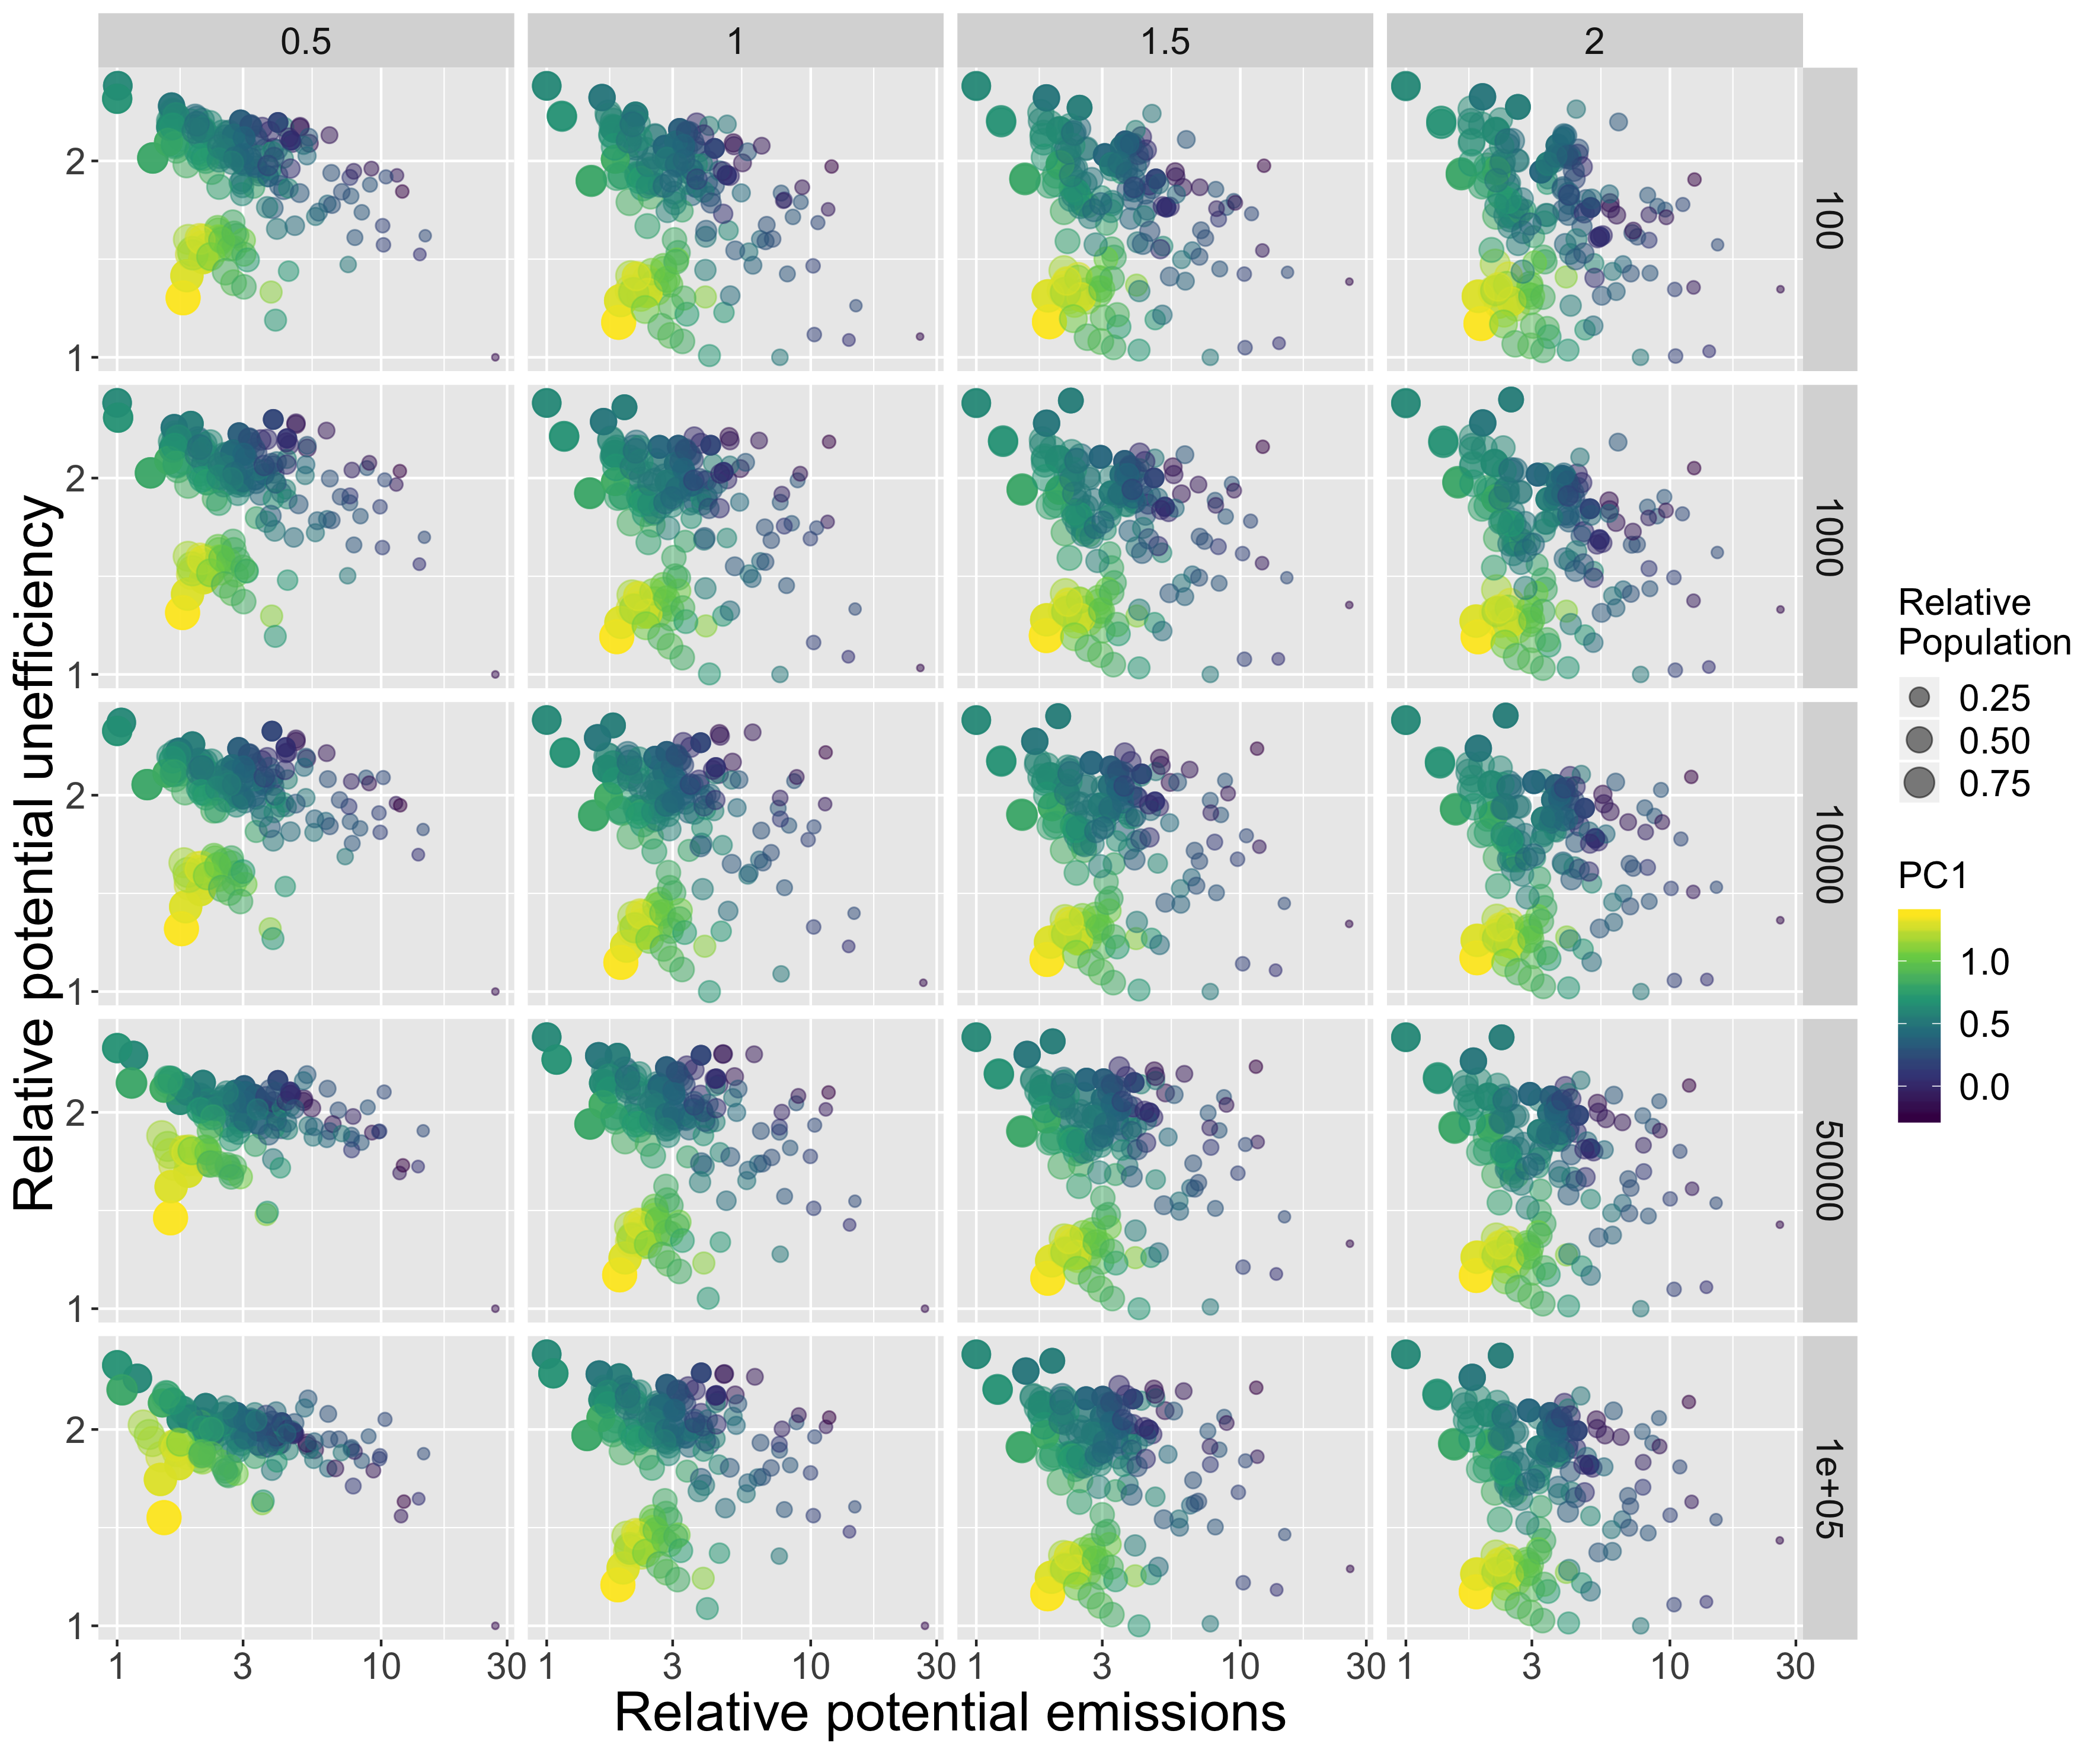
\includegraphics[width=0.49\textwidth]{figures/aggreg_morpho_relemissions-relefficiency_colpc1_logscale.png}
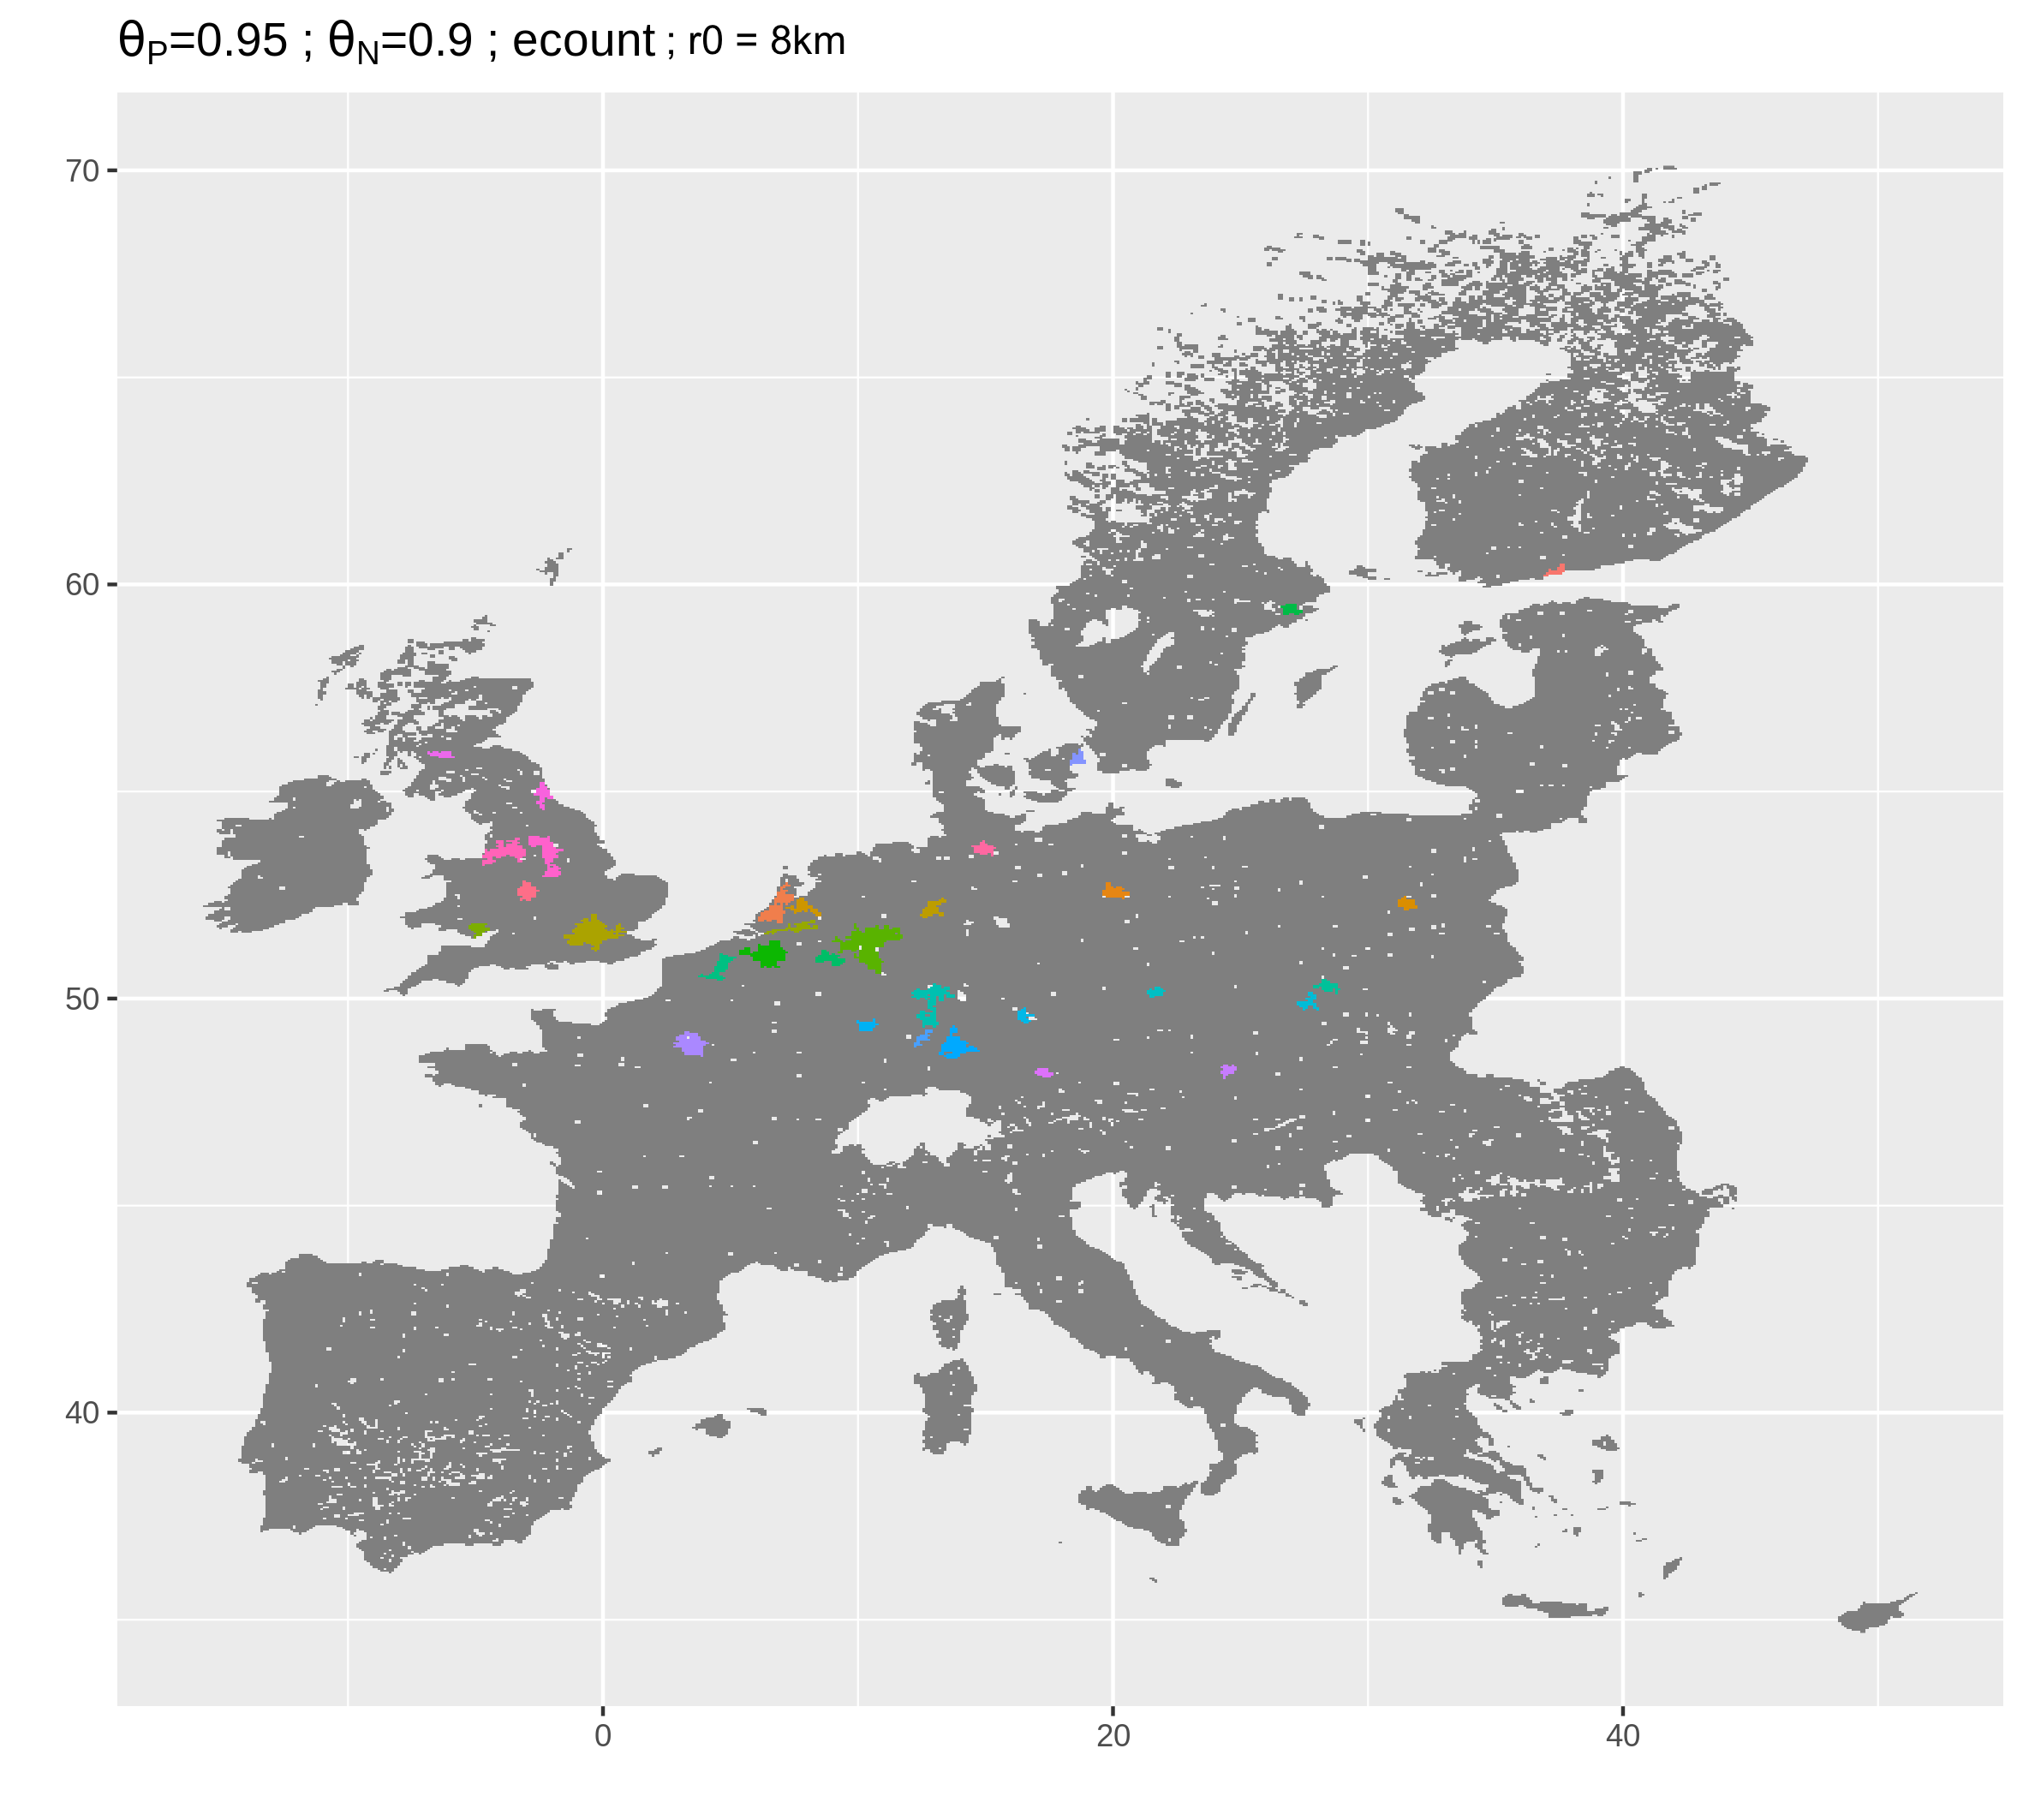
\includegraphics[width=0.49\textwidth]{figures/totalPop4183694_00056402_ecount850_radius8000.png}

\tiny

\bigskip

Raimbault, J. (2019). Multi-dimensional Urban Network Percolation. Journal of Interdisciplinary Methodologies and Issues in Sciences, 5(5).

\nocite{raimbault2019multi}

}





\sframe{Conclusion}{

\justify

$\rightarrow$ Multiple ways to model urban systems: \textbf{towards more interdisciplinary coupling and comparison of models.}

\smallskip

$\rightarrow$ At which scale? \textbf{Towards multi-scale models.}

\smallskip

$\rightarrow$ Which knowledge from simulation models? \textbf{Model exploration and validation methods.}

\smallskip

$\rightarrow$ Open question: transfer of knowledge to policies.


\bigskip

\textbf{To use OpenMOLE (free and open software) and contribute: }\\
\url{https://next.openmole.org}

\bigskip

\textbf{All models open source at }

\url{https://github.com/JusteRaimbault}




}






%%%%%%%%%%%%%%%%%%%%%
\begin{frame}[allowframebreaks]
\frametitle{References}
\bibliographystyle{apalike}
\bibliography{biblio}
\end{frame}
%%%%%%%%%%%%%%%%%%%%%%%%%%%%










\end{document}















